\documentclass{uai2023} % for initial submission
% \documentclass[accepted]{uai2023} % after acceptance, for a revised
                                    % version; also before submission to
                                    % see how the non-anonymous paper
                                    % would look like
%% There is a class option to choose the math font
% \documentclass[mathfont=ptmx]{uai2023} % ptmx math instead of Computer
                                         % Modern (has noticable issues)
% \documentclass[mathfont=newtx]{uai2023} % newtx fonts (improves upon
                                          % ptmx; less tested, no support)
% NOTE: Only keep *one* line above as appropriate, as it will be replaced
%       automatically for papers to be published. Do not make any other
%       change above this note for an accepted version.

%% Choose your variant of English; be consistent
\usepackage[american]{babel}
% \usepackage[british]{babel}

%% Some suggested packages, as needed:
\usepackage{natbib} % has a nice set of citation styles and commands
    \bibliographystyle{plainnat}
    \renewcommand{\bibsection}{\subsubsection*{References}}
\usepackage{mathtools} % amsmath with fixes and additions
% \usepackage{siunitx} % for proper typesetting of numbers and units
\usepackage{booktabs} % commands to create good-looking tables
\usepackage{tikz} % nice language for creating drawings and diagrams

%% Provided macros
% \smaller: Because the class footnote size is essentially LaTeX's \small,
%           redefining \footnotesize, we provide the original \footnotesize
%           using this macro.
%           (Use only sparingly, e.g., in drawings, as it is quite small.)

%% Self-defined macros
\newcommand{\swap}[3][-]{#3#1#2} % just an example

\title{Instructions for Authors: Title in Title Case}

% The standard author block has changed for UAI 2023 to provide
% more space for long author lists and allow for complex affiliations
%
% All author information is authomatically removed by the class for the
% anonymous submission version of your paper, so you can already add your
% information below.
%
% Add authors
\author[1]{\href{mailto:<jj@example.edu>?Subject=Your UAI 2023 paper}{Jane~J.~von~O'L\'opez}{}}
\author[1]{Harry~Q.~Bovik}
\author[1,2]{Further~Coauthor}
\author[3]{Further~Coauthor}
\author[1]{Further~Coauthor}
\author[3]{Further~Coauthor}
\author[3,1]{Further~Coauthor}
% Add affiliations after the authors
\affil[1]{%
    Computer Science Dept.\\
    Cranberry University\\
    Pittsburgh, Pennsylvania, USA
}
\affil[2]{%
    Second Affiliation\\
    Address\\
    …
}
\affil[3]{%
    Another Affiliation\\
    Address\\
    …
  }
  
  \begin{document}
\maketitle

\begin{abstract}
  This is the abstract for this article.
  It should give a self-contained single-paragraph summary of the article's contents, including context, results, and conclusions.
  Avoid citations; but if you do, you must give essentially the whole reference.
  For example: This whole paper is devoted to praising É. Š. Åland von Vèreweg's most recent book (“Utopia's government formation problems during the last millenium”, Springevier Publishers, 2016).
  Also, do not put mathematical notation and abbreviations in your abstract; be descriptive.
  So not “we solve \(x^2+A xy+y^2\), where \(A\) is an RV”, but “we solve quadratic equations in two unknowns in which a single coefficient is a random variable”.
  The reason is that mathematical notation will not display correctly when the abstract is reused on the proceedings website, for example, and that one should not assume the abstract's reader knows the abbreviation.
  Of course the same remarks hold for your paper's title.
\end{abstract}

\section{Introduction}\label{sec:intro}
UAI 2023 papers have to be prepared using \LaTeX.
To start writing your paper, copy \texttt{uai2023-template.tex} and replace title, authorship, and content with your own.

The UAI 2023 paper style is based on a custom \textsf{uai2023} class.
The class file sets the page geometry and visual style.\footnote{%
    The class uses the packages \textsf{adjustbox}, \textsf{environ}, \textsf{letltxmacro}, \textsf{geometry}, \textsf{footmisc}, \textsf{caption}, \textsf{textcase}, \textsf{titlesec}, \textsf{titling}, \textsf{authblk}, \textsf{enumitem}, \textsf{microtype}, \textsf{lastpage}, and \textsf{kvoptions}.
}
The class file also loads basic text fonts.\footnote{%
    Fonts loaded are \textsf{times} (roman), \textsf{helvet} (sanserif), \textsf{courier} (fixed-width), and \textsf{textcomp} (common symbols).
}
\emph{You may not modify the geometry or style in any way, for example, to squeeze out a little bit of extra space.}
(Also do not use \verb|\vspace| for this.)
Feel free to use convenience functionality of loaded packages such as \textsf{enumitem}.
The class enables hyperlinking by loading the \textsf{hyperref} package.

You are free to load any packages available in \TeX{Live}~2020 that are compatible with the UAI class.\footnote{In case this template or your submission does not compile, always first make sure your \TeX\ installation is up-to-date.}
(Mik\TeX{} and Mac\TeX{} generally contain the same packages.)
Do not load conflicting packages—you will get an error message—, as this complicates creating the proceedings.
Please avoid using obsolete commands, such as \verb|\rm|, and obsolete packages, such as \textsf{epsfig}.\footnote{%
    See \url{https://ctan.org/pkg/l2tabu}.
}

\swap[ ]{in the header of your source file.}{Feel free to include your own macros}

\section{General Formatting Instructions}
As a general rule: \emph{follow the template}.

\subsection{Authorship}
Reviewing is double-blind.
However, you can already fill in your author names and affiliations in the \verb|\author| block in the preamble following the example of the template because the class will remove it as long as the option \textsf{accepted} is not passed to the class.
Nevertheless, make sure any other information in the paper does not disclose your identity, for example URLs to supplementary material.

\subsection{Sectioning}
Three numbered sectioning commands are provided: \verb|\section|, \verb|\subsection|, and \verb|\subsubsection|.
Please respect their order, so do not put a \verb|\subsubsection| directly beneath a \verb|\section|.
One unnumbered sectioning command is provided, \verb|\paragraph|.
It can be used directly below any numbered section level.
Do not use any other sectioning commands.

\subsubsection{Typing the Section Titles}
The \verb|\section| and \verb|\subsection| titles are uppercased by the class.
Please type them in title case.
(This is used in the PDF bookmarks.)
Please also write the \verb|\subsubsection| titles in title case.

\paragraph{What is title case?}
\href{https://en.wikipedia.org/wiki/Title_case}{Wikipedia} explains:
\begin{quote}
    Title case or headline case is a style of capitalization used for rendering the titles of published works or works of art in English.
    When using title case, all words are capitalized except for ‘minor’ words (typically articles, short prepositions, and some conjunctions) unless they are the first or last word of the title.
\end{quote}

\subsection{References, Citations, Footnotes}\label{sec:etc}
\subsubsection{Cross-Referencing}
Always use \verb|\label| and \verb|\ref|—or a command with a similar effect—when cross-referencing.
For example, this subsection is Section~\ref{sec:etc}.

\subsubsection{Citations}
Citations should include the author's last name and year.
They should be part of the sentence.
An example parenthetical citation: “Good introductions to the topic are available \citep{latexcompanion}.”
An example textual citation: “\citet{einstein} discusses electrodynamics of moving bodies.”
Do not use a parenthetical citation where a textual one is appropriate.
An example of what \emph{not} to do: “\citep{einstein} discusses electrodynamics of moving bodies.”

We strongly advise to use reference list software such as Bib\TeX{} and a citation package such as \textsf{natbib}.
The reference style you use should be compatible with the author-year citations.
Both the citation style and reference style used should be consistent.

For the original submission, take care not to reveal the authors' identity through the manner in which one's own previous work is cited.
For example, writing
“I discussed electrodynamics of moving bodies before \citep{einstein}.” would be inappropriate, as it reveals the author's identity.
Instead, write “\citet{einstein} discussed electrodynamics of moving bodies.”

\subsubsection{Footnotes}
You can include footnotes in your text.\footnote{
    Use footnotes sparingly, as they can be distracting, having readers skip back and forth between the main text and the foot of the page.
}
The footnote mark should follow the fragment to which it refers, so a footnote\footnote{
    A footnote is material put at the foot of a page.
}
for a word has a footnote mark attached to that word and a footnote for a phrase or sentence has a footnote mark attached to the closing punctuation.

\section{Math}\label{sec:math}
The class file does not load any math support package like \textsf{amsmath}\footnote{%
  See the \textsf{amsmath} documentation at \url{https://ctan.org/pkg/amsmath} for further details.
}.
We advise using the \textsf{mathtools}\footnote{%
  See the \textsf{mathtools} documentation at \url{https://ctan.org/pkg/mathtools} for further details.
}
package, which extends \textsf{amsmath} with fixes and even more useful commands.
Feel free to load other support packages for symbols, theorems, etc.

Use the \textsf{amsmath} environments for displayed equations.
So, specifically, use the \texttt{equation} environment instead of \verb|$$...$$| and the \texttt{align} environment instead of \texttt{eqnarray}.\footnote{For reasons why you should not use the obsolete \texttt{eqnarray} environment, see Lars Madsen, \textit{Avoid eqnarray!} TUGboat 33(1):21--25, 2012.}
An \texttt{equation}:
\begin{equation}\label{eq:example}
  0 = 1 - 1.
\end{equation}
Two \texttt{align}'ed equations:
\begin{align*} % no numbers with starred version
  1 + 2 &= 3,\\
  1 - 2 &= -1.
\end{align*}
Equations can also be put inline, of course.
For example, Equation~\eqref{eq:example}: \(0=1+1\). % $0=1+1$ also works
(Notice that both inline and displayed math are part of the sentence, so punctuation should be added to displayed math.)

The \textsf{amsmath} and \textsf{mathtools} packages provide a lot of nice functionality, such as many common math operators, e.g., \(\sin\) and \(\max\), and also commands for defining new ones.

\section{Floats}\label{sec:floats}
Floats, such as figures, tables and algorithms, are moving objects and are supposed to float to the nearest convenient location.
Please do not force them to go in the middle of a paragraph.
They must respect the column width.

Two-column floats are possible.
They appear at the top of the next page, so strategic placement may be necessary.
For an example, see Figure~\ref{fig:tikz}.
They may not enter the margins.
\begin{figure*}
    \centering
    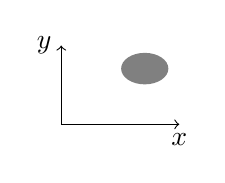
\begin{tikzpicture}[xscale=1.5]
        \coordinate (origin);
        \draw[->] (origin) -- +(1cm,0) node[below] {$x$};
        \draw[->] (origin) -- +(0,1cm) node[left] {$y$};
        \fill[gray] (45:1cm) circle[radius=.2cm];
    \end{tikzpicture}
    \caption{A Nice Filled Ellipse with a Pair of Coordinate Axes.}\label{fig:tikz}
\end{figure*}

All material in floats should be legible and of good quality.
So avoid very small or large text and pixelated or fuzzy lines.

\subsection{Figures}\label{sec:figures}
Figures should go in the \texttt{figure} environment and be centered therein.
The caption should go below the figure.
Use \verb|\includegraphics| for external graphics files but omit the file extension.
Supported formats are \textsf{pdf} (preferred for vector drawings and diagrams), \textsf{png} (preferred for screenshots), and \textsf{jpeg} (preferred for photographs).
Do not use \verb|\epsfig| or \verb|\psfig|.
If you want to scale the image, it is better to use a fraction of the line width rather than an explicit length.
For example, see Figure~\ref{fig:pitt}.

\begin{figure}[!htb]
  \centering
  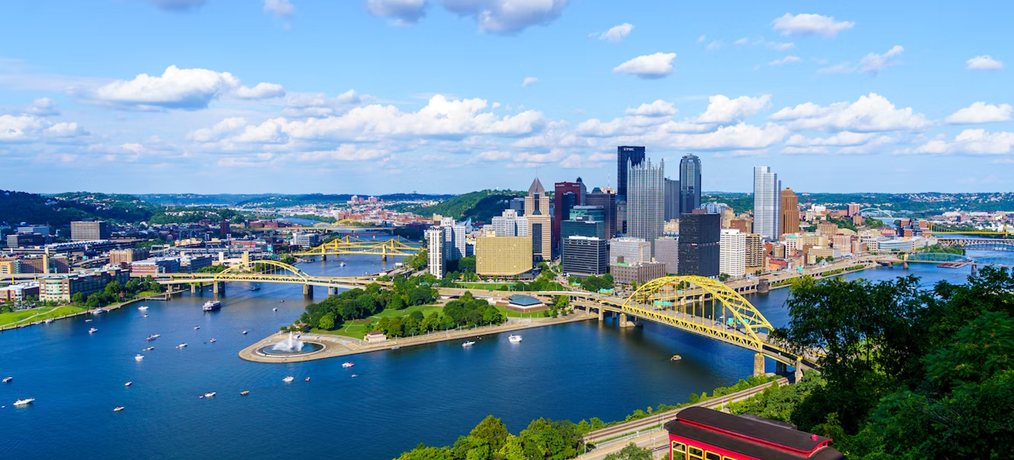
\includegraphics[width=0.7\linewidth]{pitt}
  \caption{A View of a Nice City.}\label{fig:pitt}
\end{figure}

Do not use \verb|\graphicspath|.
If the images are contained in a subdirectory, specify this when you include the image, for example \verb|\includegraphics{figures/mypic}|.

\subsection{Tables}\label{sec:tables}
Tables should go in the \texttt{table} environment and be centered therein.
The caption should go above the table and be in title caps.
For an example, see Table~\ref{tab:data}.
\begin{table}
    \centering
    \caption{An Interesting Table.}\label{tab:data}
    \begin{tabular}{rl}
      \toprule % from booktabs package
      \bfseries Dataset & \bfseries Result\\
      \midrule % from booktabs package
      Data1 & 0.12345\\
      Data2 & 0.67890\\
      Data3 & 0.54321\\
      Data4 & 0.09876\\
      \bottomrule % from booktabs package
    \end{tabular}
\end{table}

\subsection{Algorithms}\label{sec:algorithms}
You can load your favorite algorithm package, such as \textsf{algorithm2e}\footnote{See the \textsf{algorithm2e} documentation at \url{https://ctan.org/pkg/algorithm2e}.}.
Use the environment defined in the package to create a centered float with an algorithm inside.

\section{Back Matter}
There are a some final, special sections that come at the back of the paper, in the following order:
\begin{itemize}
  \item Author Contributions (optional)
  \item Acknowledgements (optional)
  \item References
\end{itemize}
They all use an unnumbered \verb|\subsubsection|.

For the first two special environments are provided.
(These sections are automatically removed for the anonymous submission version of your paper.)
The third is the ‘References’ section.
(See below.)

(This ‘Back Matter’ section itself should not be included in your paper.)


\begin{contributions} % will be removed in pdf for initial submission 
					  % (without ‘accepted’ option in \documentclass)
                      % so you can already fill it to test with the
                      % ‘accepted’ class option
    Briefly list author contributions. 
    This is a nice way of making clear who did what and to give proper credit.
    This section is optional.

    H.~Q.~Bovik conceived the idea and wrote the paper.
    Coauthor One created the code.
    Coauthor Two created the figures.
\end{contributions}

\begin{acknowledgements} % will be removed in pdf for initial submission,
						 % (without ‘accepted’ option in \documentclass)
                         % so you can already fill it to test with the
                         % ‘accepted’ class option
    Briefly acknowledge people and organizations here.

    \emph{All} acknowledgements go in this section.
\end{acknowledgements}

% References
\bibliography{uai2023-template}
\end{document}
